\chapter{Discussion \& Conclusions}

% --------------------------------------------------------------

\section{Discussion}
\subsection{Calibration with SNe-Ia Dataset}
Before analyzing the performance of Variable Chaplygin Gas Model with Gravitational Merger Event, it has to be calibrated with respect to the SCP Union Type Ia supernovae data to compare the results of the model generated to the previous published results on the model to provide credibility to the model performance on Merger events.
Variable Chaplygin Model has a provided a best fit to the SNe-Ia dataset for $\Omega_{m}$ = 0.15 and n = 0.79 with a $\chi^{2}$ goodness value of 566.296 for the distance modulus.
\begin{figure}[h]\centering
{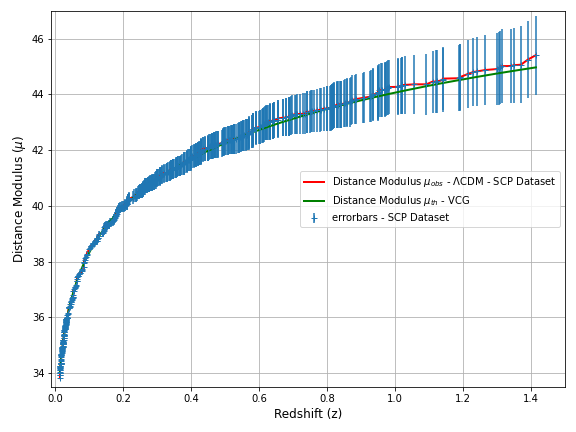
\includegraphics[width=13cm]{chap5/LCDM_DM_Redshift (1).png}
\caption{Performance of VCG Model to determine Distance Modulus (Green) with respect to the Distance Modulus from SCP Dataset (Red) against Redshift - $\Omega_{m}$=0.15, n = 0.79 and $H_{0}$=69.8}
\end{figure}

The performance VCG Model to determine luminosity distance is also included
\begin{figure}[h]\centering
{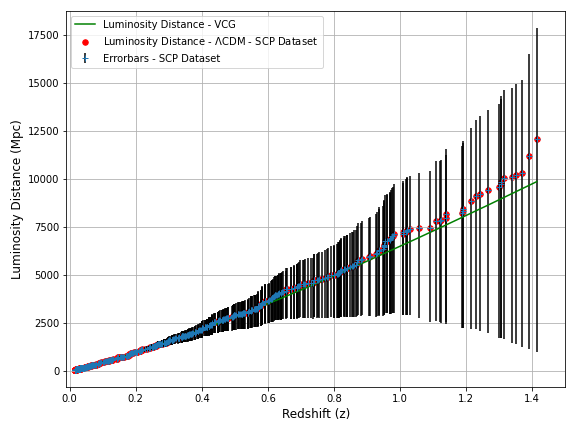
\includegraphics[width=13cm]{chap5/GoodLumi_Redshift.png}
\caption{Performance of VCG Model to determine Luminosity Distance (Green) with respect to the Luminosity Distance from $\Lambda$CDM Model (Red) against Redshift - $\Omega_{m}$=0.15, n = 0.79 and $H_{0}$=69.8}
\end{figure}

The graph depict the performance of the VCG devised against standard SCP Dataset. This provides credibility to the model has the predicted values of $\Omega_{m}$ and n closer to values from published papers: Guo & Zhong [$\Omega_{m}$=0.25, n=-2.9] and Sethi [$\Omega_{m}$=0.22, n=-2.8].
\subsection{Model performance on Gravitational Merger Events}
The Variable Chaplygin Gas Model, provided a best fit to the gravitational wave merger events obtained from GWOSC, for $\Omega_{m}$ = 0.17 and n = -8.7 with a $\chi^{2}$ goodness value of 0.388 for the distance modulus. 
\begin{figure}[h]\centering
{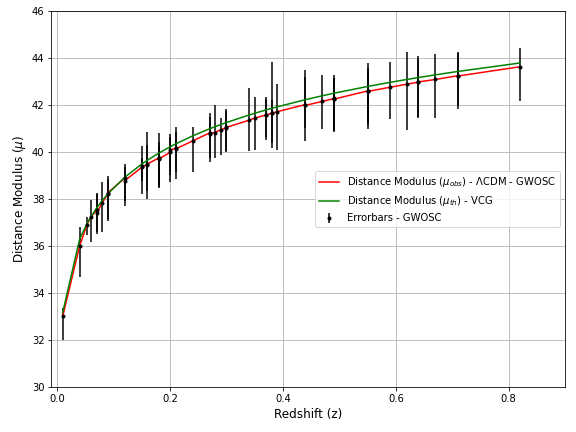
\includegraphics[width=13cm]{chap5/GW_DM.png}
\caption{Performance of VCG Model to determine Distance Modulus (Green) with respect to the Distance Modulus from $\Lambda$CDM Model (Red) against Redshift from GWOSC Dataset - $\Omega_{m}$=0.17, n = -8.7 and $H_{0}$=69.8}
\end{figure}

Similarily the perforance of VCG Model in determining Luminosity distance is given in the following plot 

\begin{figure}[h]\centering
{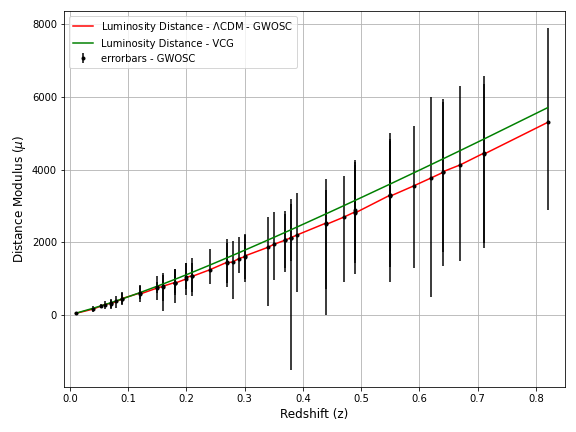
\includegraphics[width=13cm]{chap5/GW_Lumi_New.png}
\caption{Performance of VCG Model to determine Luminosity Distance (Green) with respect to the Luminosity Distance from $\Lambda$CDM Model (Red) against Redshift from GWOSC Dataset - $\Omega_{m}$=0.17, n = -8.7 and $H_{0}$=69.8}
\end{figure}

% --------------------------------------------------------------

